% https://habrahabr.ru/post/145523/
% http://fsweb.info/editors/latex/presentation.html

\documentclass[10pt]{beamer}
\usepackage[utf8]{inputenc}
\usepackage[OT1]{fontenc}
\usepackage[english, russian]{babel}
\usepackage{amsmath,amsfonts,amssymb}
\usepackage{graphicx}
%\usetheme{Singapore}
\usetheme{Berlin}

%\setbeamercolor{элемент}{bg=цвет1,fg=цвет2}. Здесь «элемент» — название элемента, чей цвет мы хотим изменить (например, «normal text» — обычный текст), «bg» — цвет фона, «fg» — цвет текста. 
%\usebackgroundtemplate{\includegraphics[width=\paperwidth,height=\paperheight]{my_backgroung_picture.jpg}}

\newcommand{\MB}{\mathbf}
\newcounter{myexmpl}
\newcounter{mypics}


\begin{document}


\title{Многоканальный органический светоизлучающий RGB диод, как элемент троичной логики}
%\subtitle{презентация по курсу}
\author{А.М. Бобрешов, А.Г. Кошелев, Е.В. Золотухин}
\institute{ВГУ}
\date{2016 год\\ 
\vspace{10mm}
{\centering

\includegraphics[scale=0.15]{pics/logo.jpg}

}}
\setbeamercovered{transparent} 
% Если в нашей презентации используется последовательное высвечивание элементов, стоит сказать: \setbeamercovered{transparent}, чтобы неактивные элементы были хотя бы немного видны.

%\setbeamertemplate{navigation symbols}{}  %убрать панель навигации

%	\author{}
	%\title{}
	%\subtitle{}
	%\logo{}
	%\institute{}
	%\date{}
	%\subject{}
	%\setbeamercovered{transparent} % или dynamic
	%\setbeamertemplate{navigation symbols}{}
	
	
%%%%%%%%%%%%%%%%%%% титул - слайд 1  %%%%%%%%%%%%%%%%%%%%%%
\begin{frame}[plain]
	%\maketitle
	  \transdissolve[duration=0.2] %добавили динамики - стиль анимированного появления страницы, где duration=0.2 - это время в секундах, за которое применяется фильтр
  \titlepage
\end{frame}

%%%%%%%%%%%%%%%%%%%%%%%% содержание - слайд 2 %%%%%%%%%%%%%%%%%%%%%%%%%%%%%%%%

\begin{frame}
  \transdissolve[duration=0.2]
  \frametitle{Содержание}
  \tableofcontents
\end{frame}

%%%%%%%%%%%%%%%%%%%%%%%%%%%%%%%%%%%%%%%%%%%%%%%%%%%%%%%%%%%%%%%%%%%%%
\section{Введение}

%%%%%%%%%%%%%%%%%%%%%%%%%%  слайд 3 %%%%%%%%%%%%%%%%%%%%%%%%%%%%

\begin{frame}[shrink=8]
\transdissolve[duration=0.2] 
\frametitle{Троичная система счисления}
Выделяют следующие методологические положения синергетики, принципиально важные для формирования синергетических основ современной прикладной теории управления:
\begin{block}{}
	Переход к цифровым методам и устройствам обработки, хранения и передачи видеоинформации, обусловленный, прежде всего, прогрессом в области создания новых технологий производства высокоэффективных изделий электронной техники, позволил значительно улучшить качество воспроизводимого изображения, увеличить число телевизионных программ, расширить диапазон исследований в области создания телевизоров и дисплеев нового поколения, включая трехмерные.
	
	Однако наряду с повышением техническо-экономических характеристик вышеупомянутых устройств существенно возрос и объем обрабатываемой и передаваемой ими информации. Например, для обработки и передачи трехмерных изображений, содержащих в глубину экрана сотни слайсов (слоев или кадров), использование традиционной двоичной системы счисления, становится малоэффективным. Поэтому, ежегодно проводимые под эгидой IEEE тематические симпозиумы (IEEE Symposium onMultiple Valued Logic) подтверждают внимание специалистов к разработкам на основе других систем счисления, включая троичную систему. Анализ опубликованных материалов позволяет утверждать, что основные усилия на сегодняшний день сосредоточены в части построения алгоритмов обработки данных на основе троичной логики тем более, что её применение предполагается учитывать при создании квантового компьютера.
\end{block}
\end{frame} 

%%%%%%%%%%%%%%%%%%%%%%%%%%  слайд 4 %%%%%%%%%%%%%%%%%%%%%%%%%%%%
\begin{frame}
\transdissolve[duration=0.2] 
\frametitle{Синергетика + теория управления  = СТУ}
Выделяют следующие методологические положения синергетики, принципиально важные для формирования синергетических основ современной прикладной теории управления:
\begin{block}{}
\begin{equation}
f(x) = x^{\frac{n}{x}}
\end{equation}
	
где n представляется минимальным набором символов в определенной системе счисления. На рис. 1 приведен график этой функции для n = 8. Из него следует, что из целочисленных систем счисления наибольшей плотностью записи информации обладает троичная система счисления. Поэтому при одинаковом числе аппаратных элементов — инверторов, троичные ЭВМ (компьютеры) имеют большую удельную ёмкость памяти и большую удельную производительность процессора, чем двоичные компьютеры. Так, опираясь на данное утверждение, ученым МГУ Н. П. Брусенцовым, в 60х годах прошлого века был разработан первый в мире уникальный троичный компьютер.	
	


\end{block}
\end{frame} 

%%%%%%%%%%%%%%%%%%%%%%%%%%  слайд 5 %%%%%%%%%%%%%%%%%%%%%%%%%%%%

\begin{frame}[shrink=20,fragile]
\transdissolve[duration=0.2]
\begin{equation}
\frac{df(x)}{dx} = n*x^{\frac{n}{x}-2}*[1-\ln(x)]=0
\ln x = 1 \Rightarrow x = e
\end{equation}
\begin{block}{}
\begin{figure}
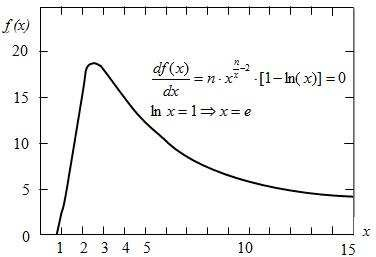
\includegraphics[scale=0.85]{pics/1.jpeg}
\caption{Функция, характеризующая компактность систем счисления по основанию x}
\end{figure}
\end{block}   

\end{frame}

%%%%%%%%%%%%%%%%%%%%%%%%%%%%%%%%%  слайд 6 %%%%%%%%%%%%%%%%%%%%%%%%%%%%%%%%%%%%%%%%%%%%%%5

\begin{frame}[shrink=20,fragile]
\transdissolve[duration=0.2]
Основные характеристики, определяющие ценность троичного кода и трехзначной логики по сравнению с двоичной логикой следующие:
\begin{block}{}
\begin{itemize}
    \item Естественное представление чисел со знаком, т.е. отсутствие приемов типа прямого, обратного, дополнительного кода.
    \item Отсутствие специального знакового бита.
    \item Сравнение значений чисел без учета знаков.
    \item Уменьшение времени для команды ветвления по знаку.
    \item Усечение длины числа равносильно правильному округлению.
    \item Троичный счетчик является реверсивным.
    \item Трехуровневый сигнал более устойчив к воздействию помех в линии передачи.
\end{itemize}
	
	Таким образом, троичное кодирование целесообразно использовать в системах приема и передачи информации, например для кодирования сигнала изображения так как, весь его спектр формируется с помощью трех основных базовых цветов – красного, зеленого и синего.
\end{block}   

\end{frame}


%%%%%%%%%%%%%%%%%%%%%%%%%%%%%%%%%  слайд 7 %%%%%%%%%%%%%%%%%%%%%%%%%%%%%%%%%%%%%%%%%%%%%%5
\begin{frame}[shrink=20,fragile]
\transdissolve[duration=0.2]
	Преимущество троичного представления данных по сравнению с двоичным можно показать на примере преобразования аналогового сигнала в цифровой код. Для этого рассмотрим и сравним динамический диапазон троичного и двоичного аналого-цифровых преобразователей (АЦП).
\begin{block}{}
	Интервал квантования определяется как:
	

	
	На основании \ref{6} и \ref{7} можно сделать вывод: для представления данных с одинаковой точностью требуется в 1,58 раза меньше троичных разрядов, чем двоичных. Снижение числа разрядов в устройстве последовательного действия за счет троичного представления данных приводит к уменьшению времени выполнения операций примерно в 1,5 раза по сравнению с двоичным кодированием, что, например, в случае матричного умножителя, обусловлено уменьшением числа последовательных сложений.
	
	Минимальная единица информации в троичной системе счислении получила название трит. Значения трита могут быть различны, например: 0,1,2 либо –1,0,+1.
	
\end{block}   
\end{frame}

\begin{frame}[shrink=20,fragile]
\transdissolve[duration=0.2]
\begin{block}{}
	Как известно, оценка качества изображения в цифровом телевидении определяется четкостью изображения (разрешением), связанной с частотой дискретизации и количеством дискретных значений (уровней квантования) относительно входного сигнала, подаваемого на вход АЦП. Иными словами разрешение АЦП — минимальное изменение величины аналогового сигнала, которое может быть преобразовано данным АЦП, что связано с его разрядностью. В случае единичного измерения без учёта шумов разрешение напрямую определяется разрядностью АЦП. Если различение соседних уровней входного сигнала становится невозможным, то разрешение ухудшается. При этом реально достижимое разрешение описывается эффективной разрядностью (effective number of bits — ENOB), которая меньше, чем реальная разрядность АЦП. При преобразовании сильно зашумленного сигнала младшие разряды выходного кода практически бесполезны, так как содержат шум.
	
	Таким образом, разрядность АЦП характеризует количество дискретных значений, которые преобразователь может выдать на выходе. На вход двоичных АЦП данные поступают в виде битов информации, а на входе троичной АЦП данные уже будут в виде тритов. В таблице 1 приведены характеристики двоичных и троичных АЦП.
\end{block}   

\end{frame}

\begin{frame}[shrink=20,fragile]
\transdissolve[duration=0.2]
\begin{block}{}

\centering	
\begin{equation}
	\delta_{2} = \frac{U_{op}}{2^{N}-1}, \delta_{3} = \frac{U_{op}}{3^{N}-1}
	\end{equation}
	
	Для двоичного и для троичного АЦП, соответственно, где   — опорное напряжение, N — разрядность АЦП. Мощности шума квантования соответственно для двоичного и для троичного АЦП имеют вид:
	
	\begin{equation}
	\bar{U^{2}_{2}} = \frac{\delta^{2}_{2}}{12},\bar{U^{2}_{3}}=\frac{\delta^{2}_{3}}{12}
	\end{equation}
	
	Среднеквадратичный шум троичного АЦП на основе формул (2) и (3) определяется как:
	
	\begin{equation}
	\label{eq4}
	\sqrt{\bar{U^{2}_{3}}}=\frac{\delta_{2}(2^{N}-1)}{2\sqrt{3}(3^{N}-1)}
	\end{equation}
	
	Максимальный сигнал для троичного АЦП есть:
	\begin{equation}
	\label{eq5}
	U_{3max}=\frac{3^{N-1}\delta_{3}}{\sqrt{1}} = \frac{3^{N-1}\delta_{2}(2^{N}-1)}{(3^{N}-1)}
	\end{equation}
	
	На основании соотношений \ref{eq4} и \ref{eq5} динамический диапазон троичного АЦП можно оценить, как:
	\begin{equation}
	DD_{3}=3^{N-1}\sqrt{6}=3^{N}\sqrt{2/3}
	\end{equation}

\end{block}   

\end{frame}

\section{Устройства троичной логики на основе многоканального RGB светодиода}
\begin{frame}[shrink=20,fragile]
\transdissolve[duration=0.2]
	Одной из проблем троичного кодирования является то, что большая часть элементов троичной логики является адаптацией элементов бинарной логики. В связи с этим в данной статье была предпринята попытка разработать троичный элемент, который работал бы непосредственно с трехуровневым сигналом. В качестве такого троичного элемента был использован многоканальный органический светоизлучающий RGB диод (воксел) в разрезе (Рис. \ref{fig2}).
	
	По принципу образования цветов в телевидении и компьютерной графике выделяют две большие группы (модели): аддитивную (RGB) и субтрактивную (CMY).
Модель RGB (Red — красный, Green — зеленый, B lue — синий) описывает излучаемые цвета. Модель CMY (C yan — голубой, M agenta — пурпурный, Y ellow — желтый) описывает отраженные цвета.
\begin{block}{}
	\begin{figure}
	\label{fig2}
	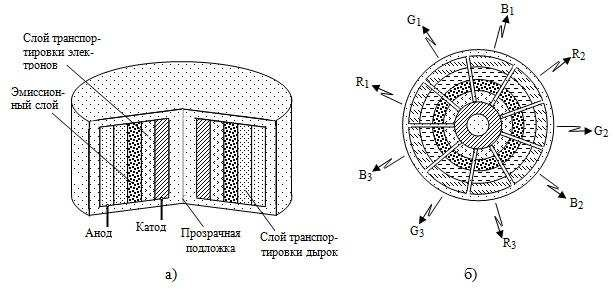
\includegraphics[scale=0.85]{pics/2.jpeg}
	\caption{Упрощенная конструкция многоканального органического RGB воксела в разрезе}
	\end{figure}
\end{block}   

\end{frame}

\begin{frame}[shrink=20,fragile]
\transdissolve[duration=0.2]

\begin{block}{}
	Так как в нашей работе в качестве формирования цвета используется светоизлучающий диод, то будем рассматривать модель RGB. Базовыми компонентами такой модели являются три цвета излучений красный, зеленый, синий. Каждому базовому цвету присваивается соответствующий тритовый символ, например, красному – (1), зеленому – (0), синему (-1) (Таблица \ref{tab2}).
Рассмотрим блок-схему и принцип действия элемента троичной логики. В качестве основы возьмем логическую операцию “И” (Таблица 3).
\begin{table}[]
\centering
\caption{Вариант кодировки цветов с помощью троичной логики}
\label{tab2}
\begin{tabular}{|l|l|l|}
\hline
Цвет    & Обозначение & Кодировка \\ \hline
Синий   & B           & 0         \\ \hline
Зеленый & G           & 1         \\ \hline
Красный & R           & 2         \\ \hline
\end{tabular}
\end{table}
	
	
\begin{table}[]
\centering
\caption{Таблица истинности для троичного логического умножения}
\label{tab3}
\begin{tabular}{|l|l|l|l|}
\hline
X\textasciicircum{}Y & 0 & 1 & 2 \\ \hline
0                    & 0 & 0 & 0 \\ \hline
1                    & 0 & 1 & 1 \\ \hline
2                    & 0 & 1 & 2 \\ \hline
\end{tabular}
\end{table}
\end{block}   

\end{frame}

\begin{frame}[shrink=20,fragile]
\transdissolve[duration=0.2]
\begin{block}{}
	Если сопоставить результаты выполнения логической функции “И” с цветовой кодировкой сигналов, то можно заметить, что в результате логического умножения двух сигналов получается сигнал, которому соответствует цвет с меньшей длиной волны. Таким образом, троичный логический элемент будет работать следующим образом: на два канала многоканального светодиода приходят сигналы, которые затем попадают на фильтр, пропускающий сигнал с большей частотой. Сигнал на выходе фильтра и будет результатом выполнения операции логического умножения. Упрощенная функциональная схема устройства представлена на Рис. \ref{fig3}.

\begin{figure}
\label{fig3}
\caption{Функциональная схема логического троичного элемента "И" на основе многоканального RGB-воксела}
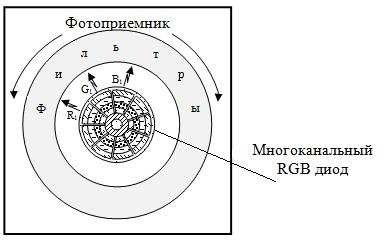
\includegraphics[scale=0.85]{pics/3.jpeg}
\end{figure}
\end{block}   

\end{frame}

\section{Варианты применения троичного кодирования}
\subsection{Работа кодирования изображения по стандарту JPEG}

\begin{frame}[shrink=20,fragile]
\transdissolve[duration=0.2]
\begin{block}{}
	В предыдущем разделе была предложена цветовая кодировка троичного сигнала. Однако остается открытым вопрос об устройстве, которое позволит передавать троичный код, закодированный цветом. Такой троичный передатчик можно построить на устройстве передачи информации, основанном на объемном многоканальном RGB светоизлучающем диоде (вокселе), способном излучать одновременно наборы красного (R), зеленого (G) и синего (B) излучения.
	
	Рассмотрим работу этого передатчика на примере кодирования изображения по стандарту JPEG. Данный стандарт относится к методам сжатия изображений с потерями и используется в основном при записи неподвижных изображений с целью экономии объема запоминающих устройств.
\end{block}   
\end{frame}

\subsubsection{Последовательность операций}

\begin{frame}[shrink=20,fragile]
\transdissolve[duration=0.2]
Последовательность операций при кодировании, поясняемая структурной схемой на рис. \ref{fig4}, включает:
—	разбиение изображения на блоки 8х8 пикселов;
—	выполнение быстрого ДКП (БДКП) в каждом блоке;
—	квантование полученных коэффициентов ДКП с использованием таблицы коэффициентов квантования (таблица Q);
—	энтропийное кодирование квантованных коэффициентов ДКП каждого блока изображения.
При этом развертка каждого блока 8х8 происходит построчно – слева направо и сверху вниз.
\begin{block}{}
\begin{figure}
\label{fig4}
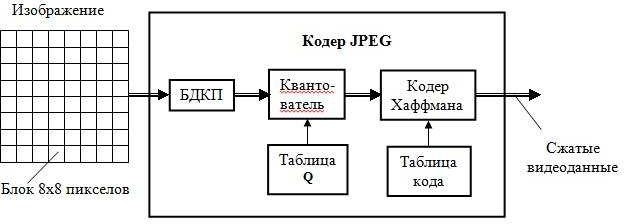
\includegraphics[scale=0.85]{pics/4.jpeg}
\caption{Структурная схема кодирования по стандарту JPEG}
\end{figure}
	Последняя операция выполняется кодером Хаффмана с использованием таблицы кодирования (таблица кодов). Вместо кодера Хаффмана может использоваться арифметический кодер.
\end{block}   
\end{frame}

\subsubsection{Обработка пикселей}
\begin{frame}[shrink=20,fragile]
\transdissolve[duration=0.2]
\begin{block}{}
	В соответствии с данным стандартом блок 8х8 пикселей развертывается построчно. Цветное изображение представляется в формате RGB, когда для каждого пиксела задаются значения трех цветов. В этом случае каждый блок 8х8 пикселов представляется тремя блоками 8х8 чисел, и каждый из них развертывается построчно. Соответственно повышается время передачи информации об изображении. За счет многоканальности воксела и троичного кодирования можно не только передавать одновременно все цвета для каждого пиксела, но можно также заменить построчную развертку одновременной разверткой сразу всех восьми строк из восьми пикселей. Каждый сегмент воксела будет отвечать за конкретный пиксел в соответствующей строке блока. Это позволит существенно сократить время, требуемое для передачи изображения.
	
	На рис. 5 показан в упрощенном виде в разрезе многоканальный RGB воксел, содержащий по 8 RGB сегментов направленных равномерно по окружности к соответствующим фотоприемникам, преобразующим свет определенного цвета и интенсивности в электрический сигнал. Далее производится троичная кодировка сигналов в соответствии с определенными цветами, например, для красного цвета (R) – (-1), для зеленого цвета (G) – (0), для синего цвета
(B)	– (+1). Затем каждый кодированный сигнал подается на вход соответствующего кодера, например, кодера JPEG. Причем, все кодированные сигналы подаются на соответствующие кодеры одновременно (Рис.\ref{fig6}).
	
	Таким образом, скорость развертки блоков кадра возрастает в 8 раз.
\end{block}   
\end{frame}

\section{Заключение}

\begin{frame}[shrink=20,fragile]
\transdissolve[duration=0.2]
\begin{block}{}
	Исходя из полученных выше результатов анализа многоканального органического светодиода кругового RGB излучения, а также целесообразности использования цветового кодирования троичного сигнала с помощью трех основных базовых цветов – красного, зеленого и синего, можно заключить следующее.
	
	Конструктивно-технологические и выходные электрические характеристики многоканального органического светодиода кругового RGB излучения (его многоканальность и круговое одновременное излучение разных длин световых волн в заданной последовательности), позволяют:
	
	Применять его для создания логических элементов на базе троичной логики.
	\begin{figure}
	\label{fig5}
	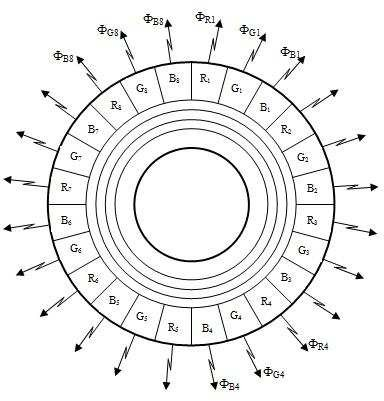
\includegraphics[scale=0.85]{pics/5.jpeg}
	\caption{Упрощенный вид сверху многоканального RGB воксела}
	\end{figure}
\end{block}   
\end{frame}

\begin{frame}[shrink=20,fragile]
\transdissolve[duration=0.2]
\begin{block}{}
	 Использовать троичный передатчик на его основе, как в беспроводной передачи данных на расстояние по оптическому каналу связи, так и по каналам межблочной связи.
	
	К основным преимуществам такого способа передачи информации можно отнести: высокие скорости передачи, простота инсталляции, а также работа в свободной области частотного диапазона.
	
	Использование цветового кодирования троичного сигнала повышает скорость и объем передаваемой информации, а также упрощает само устройство. Особенно это видно при обработке изображения по стандарту JPEG. Если воксел адаптировать к работе с троичной логикой, то можно добиться перехода от построчной развертки изображения к одновременной развертке трех и более строк. При этом основные константы троичной системы счисления 0, 1 и -1 должны кодироваться зеленым, красным и синим цветом соответственно. Таким образом, в перспективе можно получить системы передачи изображения, превосходящие современные по скорости и объему передаваемой информации.
	\begin{figure}
	\label{fig6}
	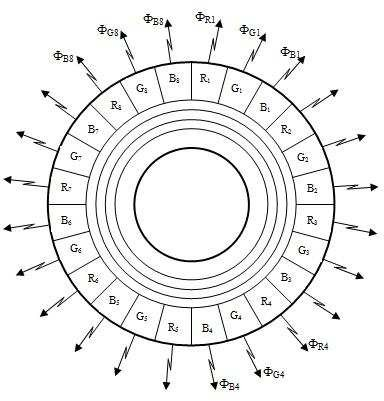
\includegraphics[scale=0.85]{pics/5.jpeg}
	\caption{Единовременная (параллельная) развертка 8 строк каждого блока RGB пикселов}
	\end{figure}
\end{block}   
\end{frame}

\end{document}